\chapter*{Dodatak: Prikaz aktivnosti grupe}
		\addcontentsline{toc}{chapter}{Dodatak: Prikaz aktivnosti grupe}
		%dd
		\section*{Dnevnik sastajanja}	
		\begin{packed_enum}
			\item  sastanak
			
			\item[] \begin{packed_item}
				\item Datum: 20.10.2022.
				\item Trajanje: 2h
			
			
				\item Prisustvovali: \begin{packed_enum}
				
				\item[]  M. C. Belušić Gonzales,
						 L. Crnković,
				  	     D. Grdić,
						 M. Pristav,
						 L. Salihović,
						 M. Vidas,
						 I. Žgela
				\end{packed_enum}
				\item Teme sastanka:
				\begin{packed_item}
					\item  Upoznavanje s zadatkaom
					\item  Izlučivanje zahtjeva aplikacije
					\item  Razriješavanje inicijalnih nedoumica
					\item  Odabir baznih tehnologija
					\item  Rasprava i opisivanje relacijskog modela baze podataka
					\item  Opisivanje osnovnog UI izgleda
					\item  Proučavanje API dokumentacije
				\end{packed_item}
			\end{packed_item}
		
		\item  sastanak
		
		\item[] \begin{packed_item}
			\item Datum: 25.10.2022.
			\item Trajanje: 3h
			
			
			\item Prisustvovali: \begin{packed_enum}
				
				\item[]  M. C. Belušić Gonzales,
				L. Crnković,
				D. Grdić,
				M. Pristav,
				L. Salihović,
				M. Vidas,
				I. Žgela
			\end{packed_enum}
			\item Teme sastanka:
			\begin{packed_item}
				\item  Upoznavanje s detaljima dokumentacije
				\item Započeta podjela posla oku dokumentacije
				\item Određeni načini praćenja rada u timu
			\end{packed_item}
		\end{packed_item}
	
		\item  sastanak
	
	\item[] \begin{packed_item}
		\item Datum: 26.10.2022.
		\item Trajanje: 1.5h
		
		
		\item Prisustvovali: \begin{packed_enum}
			
			\item[]  M. C. Belušić Gonzales,
			L. Salihović,
			I. Žgela
		\end{packed_enum}
		\item Teme sastanka:
		\begin{packed_item}
			\item  Definrian općenit dizaj i boje web stranice
			\item  Definirane komponente koje je potrebno implementirati
			\item Dogovor oko raspodjele poslova do slijedećeg sastanka
		\end{packed_item}
	\end{packed_item}
\item  sastanak

\item[] \begin{packed_item}
	\item Datum: 30.10.2022.
	\item Trajanje: 2.5h
	
	
	\item Prisustvovali: \begin{packed_enum}
		
		\item[]  L. Crnković,
		D. Grdić,
		M. Pristav,
		M. Vidas
	\end{packed_enum}
	\item Teme sastanka:
	\begin{packed_item}
		\item  Otrkriveni i prodiskutirani problemi sa spajanjem na API
		\item  Osvježen UML baze podataka
		\item  Istraživanje okolnosti našeg zadatka\newline (mogućnosti transmitera,antena,satelita...)
		\item  Istraživanje konkretnog formata potrebnih podataka
	\end{packed_item}
\end{packed_item}

\item  sastanak

\item[] \begin{packed_item}
	\item Datum: 31.10.2022.
	\item Trajanje: 1h
	
	
	\item Prisustvovali: \begin{packed_enum}
		
		\item[]  M. C. Belušić Gonzales,
		I. Žgela
		 
	\end{packed_enum}
	\item Teme sastanka:
	\begin{packed_item}
		\item  Zajedničko rješavanje konfilkata
		\item  Zajedničko rješavanje problema prijave korisnika u aplikaciju
		\item  Raspodjela zadataka i uređivnje gitlab board-a
		\item Međusobno pokazivanje koda i konzultacija za nastavak rada na aplikaciji
	\end{packed_item}
\end{packed_item}
\item  sastanak
\item[] \begin{packed_item}
	\item Datum: 2.11.2022.
	\item Trajanje: 3.5h
	
	
	\item Prisustvovali: \begin{packed_enum}
		
		\item[]  L. Crnković,
		D. Grdić,
		M. Pristav,
		M. Vidas
	\end{packed_enum}
	\item Teme sastanka:
	\begin{packed_item}
		\item  Testiranje get zahtjeva na API-ju
		\item  Planiranje daljnjeg rada backenda
		\item  Pojašnjenje novih aspekata dokumentacije
		\item  ispravljanje prijašnjih grešaka u radu i shvaćanju zadatka
		\item  Određen termin za zajedničko stvaranje dijela dokumentacija
	\end{packed_item}
\end{packed_item}

\item  sastanak

\item[] \begin{packed_item}
	\item Datum: 3.11.2022.
	\item Trajanje: 4h
	
	
	\item Prisustvovali: \begin{packed_enum}
		
		\item[]  
		L. Crnković,
		D. Grdić,
		M. Pristav,
		L. Salihović,
		M. Vidas,
		I. Žgela
	\end{packed_enum}
	\item Teme sastanka:
	\begin{packed_item}
		\item  Sastanak sa asistentom
		\item Provjera dosadašnjeg rada i uspunjenja zahtjeva zadatka
		\item Odlučen način i redovitost povezivanja na satnogs network
		\item Dovršen model baze podataka
		\item Napravljenji  dijagrami obrazaca uporabe
		\item Usklađivanje workspaceova na frontendu
		\item Dogovor oko načina predaje formi
	\end{packed_item}
\end{packed_item}
	\item  sastanak

\item[] \begin{packed_item}
	\item Datum: 10.11.2022.
	\item Trajanje: 4h
	
	
	\item Prisustvovali: \begin{packed_enum}
		
		\item[]  M. C. Belušić Gonzales,
		L. Crnković,
		D. Grdić,
		M. Pristav,
		L. Salihović,
		M. Vidas,
		I. Žgela
	\end{packed_enum}
	\item Teme sastanka:
	\begin{packed_item}
		\item  Usklađivanje frontend i backend ideja i dovršenog posla
		\item  Spajanje frontend i backend koda
		\item  Dovršavanje funkcionalnosti LogIn/LogOut
		\item  Dodavanje previđenih Obrazaca Uporabe
		\item  Zapoečta modelacija Sekvencijskih dijagrama
		\item  Zajednička provjera/pregled dijelova dokumentacije
		\item  Dodane manje preinake u bazu podataka
		\item  Raspravljene moguće promjene o finalnom načinu rada aplikacije
	\end{packed_item}
\end{packed_item}
	\item  sastanak
\item[] \begin{packed_item}
	\item Datum: 18.11.2022.
	\item Trajanje: 3h
	
	
	\item Prisustvovali: \begin{packed_enum}
		
		\item[] 
		L. Crnković,
		D. Grdić,	
		M. Vidas,
		I. Žgela
	\end{packed_enum}
	\item Teme sastanka:
	\begin{packed_item}
		\item Deployment aplikacije
		\item Testiranje deployane aplikacije
	\end{packed_item}
\end{packed_item}
%-------------------------------------------- novi sastanci
	\item  sastanak
\item[] \begin{packed_item}
	\item Datum: 19.12.2022.
	\item Trajanje: 4h
	
	
	\item Prisustvovali: \begin{packed_enum}
		
		\item[]  M. C. Belušić Gonzales,
		L. Crnković,
		D. Grdić,
		M. Pristav,
		L. Salihović,
		M. Vidas,
		I. Žgela
	\end{packed_enum}
	\item Teme sastanka:
	\begin{packed_item}
		\item Osvrt na demonstraciju alfa inačice
		\item Raspodjela preostale implementacije nakon sastanka s asistentom
		\item Postavljen rok za dovršetak implementacije i početak dokumentacije
		\item Dogovoren termin sljedećeg sastanka
		
	\end{packed_item}
\end{packed_item}
	\item  sastanak
\item[] \begin{packed_item}
	\item Datum: 5.1.2023.
	\item Trajanje: 2h
	
	
	\item Prisustvovali: \begin{packed_enum}
		
		\item[]  M. C. Belušić Gonzales,
		L. Crnković,
		D. Grdić,
		M. Pristav,
		L. Salihović,
		M. Vidas,
		I. Žgela
	\end{packed_enum}
	\item Teme sastanka:
	\begin{packed_item}
		\item Zajednički pregled funkcionalnosti aplikacije
		\item Pregled potrebnih znanja za daljnju dokumentaciju
		\item Raspodjela posla oko dokumentacije
		\item Predložene manje promjene u dizajnu aplikacije
		
		
	\end{packed_item}
\end{packed_item}



%

\end{packed_enum}

\eject
\section*{Tablica aktivnosti}

\begin{longtblr}[
label=none,
]{
	vlines,hlines,
	width = \textwidth,
	colspec={X[7, l]X[1, c]X[1, c]X[1, c]X[1, c]X[1, c]X[1, c]X[1, c]}, 
	vline{1} = {1}{text=\clap{}},
	hline{1} = {1}{text=\clap{}},
	rowhead = 1,
} 
\SetCell[c=1]{c}{} & 	\SetCell[c=1]{c}{\rotatebox{90}{\textbf{Mihael Pristav}}} & 	\SetCell[c=1]{c}{\rotatebox{90}{\textbf{Maria Carmen Belušić Gonzales }}} &		\SetCell[c=1]{c}{\rotatebox{90}{\textbf{Leticija Crnković}}} & 	\SetCell[c=1]{c}{\rotatebox{90}{\textbf{Dalen Grdić }}} &		\SetCell[c=1]{c}{\rotatebox{90}{\textbf{Leona Salihović }}} & 	\SetCell[c=1]{c}{\rotatebox{90}{\textbf{Marta Vidas }}} &		\SetCell[c=1]{c}{\rotatebox{90}{\textbf{Ivan Žgela }}} \\  
Opis projektnog zadatka 	& 1 &5  &  &  &  &  & \\ 

Funkcionalni zahtjevi       &1  &  &  & & 2 &0.5  &  \\ 
Opis pojedinih obrazaca 	&11  &  &  &  & 2.5 &2  & 0.5 \\ 
Dijagram obrazaca 			&1.5  &  &  &  &  & &  \\
Sekvencijski dijagrami 		&1  &  &  &  &  &  &  \\ 
Opis ostalih zahtjeva 		&  &  &  &  &  &0.5  &  \\ 

Arhitektura i dizajn sustava	 &  &  &  &  &  &0.5 &  \\ 
Baza podataka				&2  &  &  &  &  & 4.5 & 2.5  \\ 
Dijagram razreda 			&  &  &1.5  &  &  &0.5  &   \\ 
Dijagram stanja				&  &  &  &  &  &  &2  \\ 
Dijagram aktivnosti 		&  &  &1  &1  &  &  &  \\ 
Dijagram komponenti			&  &  &  & 1 &  &1  &  \\ 
Korištene tehnologije i alati 		&0.5  &  &  &  &2  &  &  \\ 
Ispitivanje programskog rješenja 	&1  &2.5  &  &  &  &1  &  \\ 
Dijagram razmještaja			&  &  &  &  &1  &  &  \\ 
Upute za puštanje u pogon 		&  &  &4  &  &  &  &  \\  
Dnevnik sastajanja 			&2  &  &  &  &  &  &0.5  \\ 
Zaključak i budući rad 		&  &  &  &  &2  &  &  \\  
Popis literature 			&1  &  &  &  &  &  &  \\  
\textbf{Ukupno dokumentacija}	&22  &7.5  &6.5  &2  &9.5  & 10.5 &5.5  \\ 
 
\textit{Upravljanje projektom} 		& 11 &  &  &  &  &  & \\
\textit{back end} 							&24  &  &17  &30  &  &36  &  \\  
\textit{front end} 							&  &28  &  &  & 22 &  & 42 \\  

\textit{deployment} 							&  &4  &17  &15  &5  &10  &3  \\
\textit{Istraživanje informacija/tehnologija} 				&10  &12  &7.5  &7.5  &10  &6.5  &11 
\\
%tu sam odlučilpisati kolko vremena je otišlo napodešavanje-/popravljanje te njihove blesave skripte u latecu + proucavanje materjala za dokumentaciju iskreno nisam znal kad drugdje to zapisat
\textit{izrada baze podataka} 		 			&2  &  &1  &1  &  &1  & \\ 
\textit{izrada dijagrama} 		 			&10  & 3.5 &8  &11.5  &3  &7  &4 \\ 
\textit{izrada dizajna aplikacije u Figmi} 		 			&  &  &  &  & 6 &  & \\

\textbf{Ukupno razvoj projekta}	&79  &55 &57 &67 &55.5 &71 & 65.5 \\\end{longtblr}
					
					
		\eject
		\section*{Dijagrami pregleda promjena}
		
		 \begin{figure}[H]
			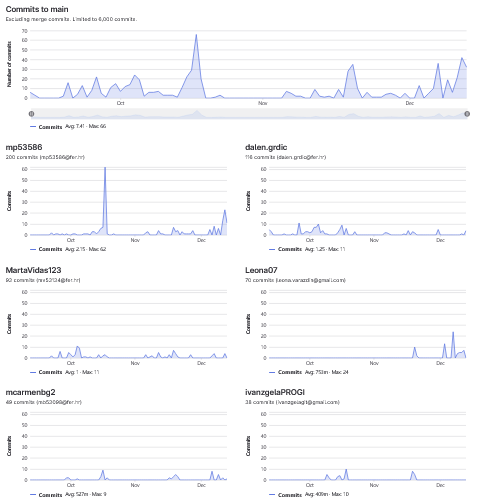
\includegraphics[width=\linewidth]{grafComitova.png}
			\caption{Graf gitLab aktivnosti}
			\label{fig:DijagramGitlaba}
		\end{figure}
	\begin{figure}[H]
		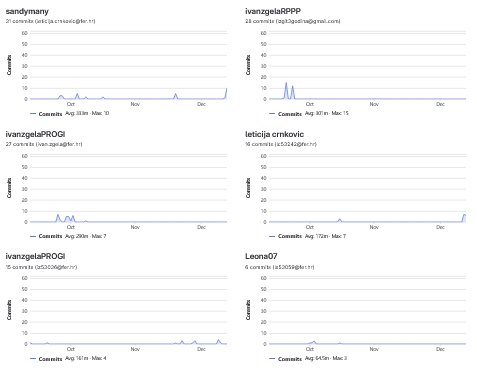
\includegraphics[width=\linewidth]{grafComitova2.png}
		\caption{Graf gitLab aktivnosti-nastavak}
		\label{fig:DijagramGitlaba2}
	\end{figure}
		
	
